\subsection{Circle parametric equation}

\begin{table}[ht]
	\begin{center}
		\begin{tabular}[top]{ |p{16.0 cm}| }
			\rowcolor{LIGHTCYAN}			
		%%	\hline \multicolumn{1}{|c|}{\textbf{Part 3/5 Circle and AstEpi parametric curves}} \\ [1.0ex]

			\hline \textbf{No. 5 - Circle parametric curve} \\
			\begin{eqnarray}
				x(u) & = & 79\sin(2\pi u) \nonumber \\   
				y(u) & = & 79\cos(2\pi u) \nonumber \\
				u & \in & [0.0, 1.0] \nonumber
			\end{eqnarray}
			
			Closed loop\\
			Overall Single loop, smooth convex curves\\
			Reflection x-axis: symmetrical\\
			Reflection y-axis: symmetrical\\
			\frame{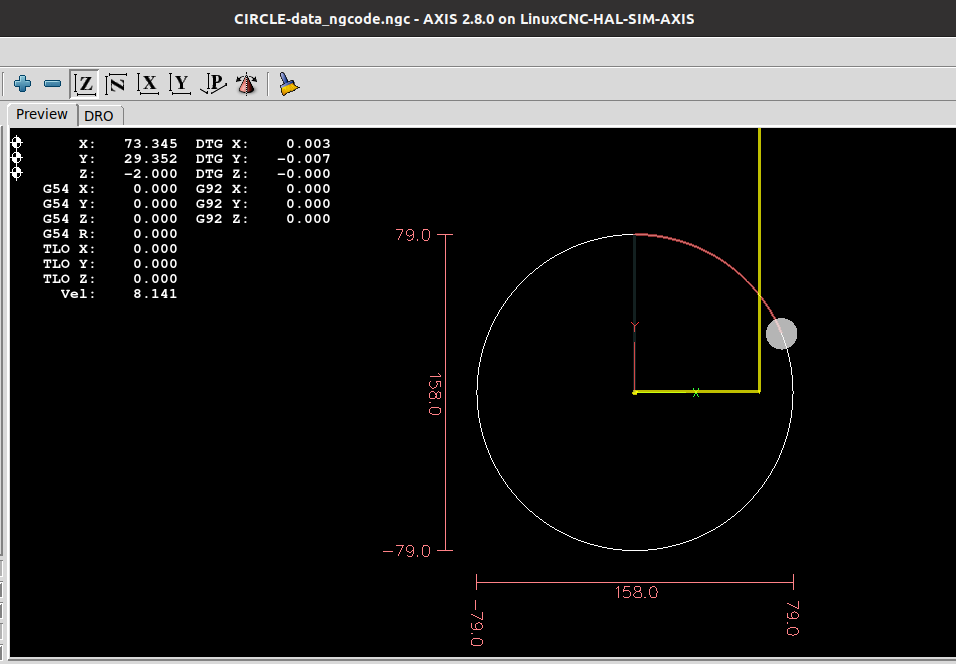
\includegraphics[width=0.560\textwidth]{./07-images/img-Ch5/CIRCLE-Axis.png}}
			\frame{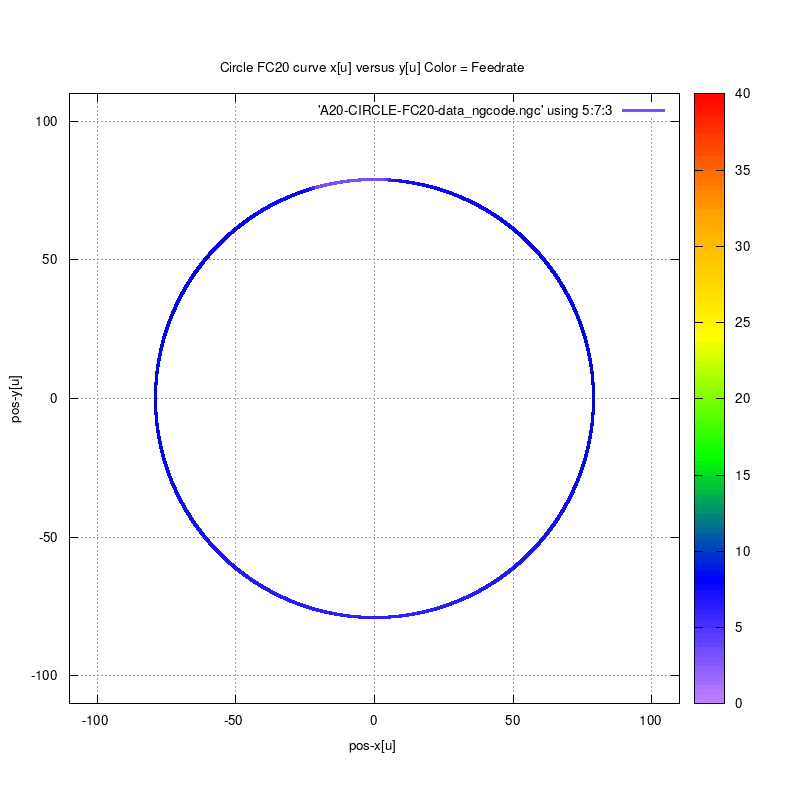
\includegraphics[width=0.394\textwidth]{./07-images/img-Ch5/CIRCLE-Feedrate.png}}\\
			
           
			\hline
		\end{tabular}
		\caption{Circle equation and dimensions}		
		\label{table:Circle equation and dimensions}
	\end{center}
\end{table}  
